\documentclass[12pt]{article}
\def\activityid{F05-U-v3}\usepackage[letterpaper,margin=.65in,top=.60in,bottom=.65in]{geometry}
\usepackage[T1]{fontenc}\usepackage[default]{sourcesanspro}
\usepackage{microtype,tikz,array,tabularx,fancyhdr,amsmath}\usepackage[hidelinks]{hyperref}
\usetikzlibrary{arrows.meta,calc}
\setlength{\parindent}{0pt}\setlength{\parskip}{7pt}\setlength{\headheight}{0pt}\setlength{\footskip}{26pt}\setlength{\emergencystretch}{2em}
\pagestyle{fancy}\fancyhf{}\renewcommand{\headrulewidth}{0pt}\renewcommand{\footrulewidth}{.4pt}
\fancyfoot[L]{\scriptsize Bellingham Math Circle / Week 5 / \activityid}\fancyfoot[R]{\scriptsize \thepage}
\definecolor{ink}{gray}{.12}\definecolor{soft}{gray}{.95}\color{ink}
\newcommand{\PageTitle}[2]{{\fontsize{10}{12}\selectfont\bfseries WEEK 5\quad TOWER LAB\hfill #1\par}\vspace{3pt}{\fontsize{26}{29}\selectfont\bfseries #2\par}\vspace{2pt}}
\newcommand{\Subhead}[1]{\par\vspace{3pt}{\large\bfseries #1}\par}
\newcommand{\RuleBox}[1]{\par\begingroup\setlength{\fboxsep}{8pt}\colorbox{soft}{\parbox{\dimexpr\linewidth-16pt\relax}{#1}}\endgroup\par}
\newcommand{\WriteBox}[2]{\par\textbf{#1}\par\vspace{2pt}\begin{tikzpicture}\draw[black!40,line width=.5pt] (0,0) rectangle (\dimexpr\linewidth-.5pt\relax,#2);\end{tikzpicture}\par}
\newcommand{\Code}[1]{\texttt{#1}}

\newcommand{\StudentHeader}[1]{{\fontsize{10}{12}\selectfont\bfseries Week 5 / Tower lab / #1\par}\vspace{10pt}}
\newcommand{\Problem}[2]{\par\vspace{4pt}\textbf{Problem #1:} #2\par}
\newcommand{\RecordBox}[2]{\par #1\par\vspace{2pt}\begin{tikzpicture}\draw[black!40,line width=.5pt](0,0)rectangle(\dimexpr\linewidth-.5pt\relax,#2);\end{tikzpicture}\par}

\hypersetup{pdftitle={Week 5: Grades 4--5}}
\begin{document}
\StudentHeader{Grades 4--5}
\Problem{1}{Build these rows with heights 1, 2, 3, and 4. Look from both ends. Count visible towers; a taller tower hides any shorter tower behind it.}
\begin{center}\renewcommand{\arraystretch}{1.65}\begin{tabular}{c|c|c}Order, left to right & Seen left & Seen right\\\hline
1 4 2 3 &  & \\
2 1 4 3 &  & \\
4 1 2 3 &  & \\
4 2 1 3 &  & \\\end{tabular}\end{center}
\Problem{2}{Build a city using heights 1--4 once in every row and once in every column. Each outside number counts towers seen from that end. Solve the city below and record each tower height.}
\begin{center}\begin{tikzpicture}[x=0.6in,y=0.6in]\draw[step=1,black!55](0,0)grid(4,4);\draw[thick](0,0)rectangle(4,4);\node at(-0.45,1.5){2};\node at(-0.45,0.5){1};\node at(4.45,2.5){2};\node at(4.45,1.5){2};\node at(4.45,0.5){2};\node at(-0.45,3.5){4};\node at(0.5,4.45){4};\end{tikzpicture}\end{center}
\RecordBox{One tower I placed and the clue I used:}{0.55in}

\newpage
\StudentHeader{Grades 4--5}
\Problem{3}{Remove the top clue 4 and the left clue 4. Rebuild using only the five remaining clues below. Keep a record of any different city you find.}
\begin{center}\begin{tikzpicture}[x=0.61in,y=0.61in]\draw[step=1,black!55](0,0)grid(4,4);\draw[thick](0,0)rectangle(4,4);\node at(-0.45,1.5){2};\node at(-0.45,0.5){1};\node at(4.45,2.5){2};\node at(4.45,1.5){2};\node at(4.45,0.5){2};\end{tikzpicture}\end{center}
\Problem{4}{Use four towers to test bottom rows before filling the city. Record every bottom row that shows one tower from the left and two from the right. Keep both possibilities available.}
\RecordBox{Possible bottom rows, left to right:}{0.75in}
\Problem{5}{Now build rows showing two towers from each end. Record all the different rows you find. These are candidates for row 3, counting rows from the top.}
\RecordBox{Possible row 3 orders:}{0.75in}

\newpage
\StudentHeader{Grades 4--5}
\Problem{6}{Pair each bottom row from Problem 4 with each row 3 from Problem 5. Reject a pair if a column repeats a height. Record the pairs that survive. For each pair, try every row 2 that avoids column repeats and shows two towers from the right. Write all the row 2 orders that work, or write ``none.''}
\begin{center}\renewcommand{\arraystretch}{3}\begin{tabular}{p{1.6in}|p{1.6in}|p{2.5in}}Bottom row & Row 3 & Row 2 orders that work\\\hline
 &  & \\
 &  & \\
 &  & \\\end{tabular}\end{center}
\Problem{7}{For each case that survives Problem 6, fill the top row with the heights missing from its columns. Record the completed city. Check all five clues again.}
\begin{center}\begin{tikzpicture}[x=0.6in,y=0.6in]\draw[step=1,black!55](0,0)grid(4,4);\draw[thick](0,0)rectangle(4,4);\node at(-0.45,1.5){2};\node at(-0.45,0.5){1};\node at(4.45,2.5){2};\node at(4.45,1.5){2};\node at(4.45,0.5){2};\end{tikzpicture}\end{center}

\newpage
\StudentHeader{Grades 4--5}
\Problem{8}{Start with the five-clue city from Problem 7. Cover the left clue on row 3. Try to make a different city that keeps the other four clues. Record it, then restore the covered clue.}
\begin{center}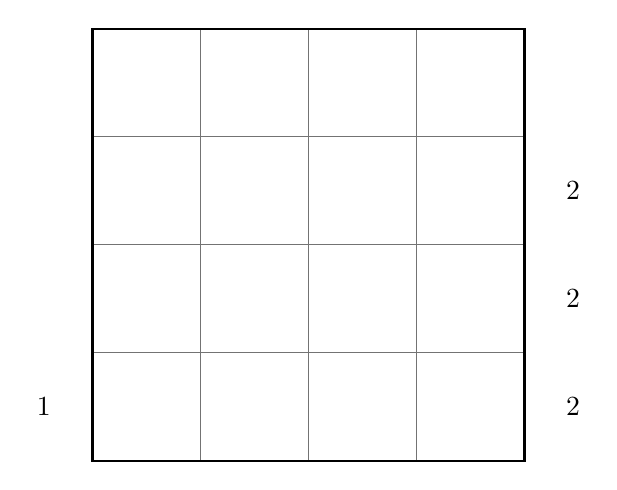
\begin{tikzpicture}[x=0.54in,y=0.54in]\draw[step=1,black!55](0,0)grid(4,4);\draw[thick](0,0)rectangle(4,4);\node at(-0.45,0.5){1};\node at(4.45,2.5){2};\node at(4.45,1.5){2};\node at(4.45,0.5){2};\end{tikzpicture}\end{center}
\Problem{9}{Check the alternatives below one at a time. L3 means the left clue on row 3; R2 means the right clue on row 2. In each city, a slash begins the next row, from top to bottom. Check every row and column and the four retained clues. Record the actual view at the covered clue. Restore it before the next check.}
\begin{center}\renewcommand{\arraystretch}{1.7}\begin{tabular}{c|p{3.9in}|c}Cover & Alternative city & Actual view\\\hline
L3 & 1234 / 3412 / 2341 / 4123 & \\
L4 & 1234 / 4123 / 3412 / 2341 & \\
R2 & 1324 / 2431 / 3142 / 4213 & \\
R3 & 1324 / 3142 / 2431 / 4213 & \\
R4 & 1234 / 2143 / 3412 / 4321 & \\\end{tabular}\end{center}

\newpage
\StudentHeader{Grades 4--5}
\Problem{10}{Remove every old clue. Use only left clues 4, 3, and 2 on rows 1, 2, and 3. Build a city with these clues and record its tower heights.}
\begin{center}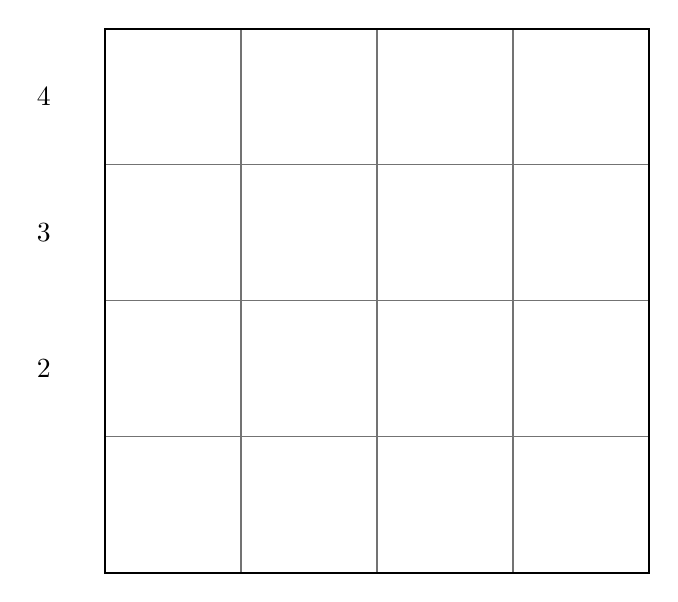
\begin{tikzpicture}[x=0.68in,y=0.68in]\draw[step=1,black!55](0,0)grid(4,4);\draw[thick](0,0)rectangle(4,4);\node at(-0.45,3.5){4};\node at(-0.45,2.5){3};\node at(-0.45,1.5){2};\end{tikzpicture}\end{center}
\Problem{11}{List the top rows that work with its clue. Then list the row 2 orders that fit its clue and avoid repeats under the top row. Continue with row 3. Fill row 4 with each column's missing height.}
\begin{center}\renewcommand{\arraystretch}{2}\begin{tabular}{c|p{5.7in}}Row & Orders that fit all earlier rows and this row's clue\\\hline
1 & \\
2 & \\
3 & \\
4 & \\\end{tabular}\end{center}
\Problem{12}{Compare this city with your five-clue city. Record how many clues each puzzle used and whether the completed cities agree.}
\RecordBox{My comparison:}{0.5in}

\end{document}
